\documentclass[12pt]{article}
%\documentclass[12pt,legalpaper]{article}
%\documentclass[14pt,legalpaper]{extarticle}
\usepackage{fullpage}
\usepackage{amsmath,amssymb}
\usepackage{mathptmx}
\usepackage{fancyhdr}
\usepackage{lastpage}
\usepackage{multicol}
\usepackage{graphicx}
\usepackage[aux]{rerunfilecheck}
\usepackage[rflt]{floatflt}

%\setlength{\textheight}{11.5in}

\reversemarginpar

\newcommand{\myimp}{\Rightarrow}
\newcommand{\myiff}{\Leftrightarrow}
\newcommand{\mynot}{\neg}
\newcommand{\myor}{\vee}
\newcommand{\myand}{\wedge}
\newcommand{\ds}{\displaystyle}

\DeclareSymbolFont{AMSb}{U}{msb}{m}{n}
\DeclareMathSymbol{\N}{\mathbin}{AMSb}{"4E}
\DeclareMathSymbol{\Z}{\mathbin}{AMSb}{"5A}
\DeclareMathSymbol{\R}{\mathbin}{AMSb}{"52}
\DeclareMathSymbol{\Q}{\mathbin}{AMSb}{"51}
\DeclareMathSymbol{\I}{\mathbin}{AMSb}{"49}
\DeclareMathSymbol{\C}{\mathbin}{AMSb}{"43}

\pagestyle{fancy}
\lhead{MATH 110 200730                                                     \\ 
  Final Examination \hspace{1.25in} Page\ \thepage\ of \pageref{LastPage}  \\ 
  Time: 3 hours                                                            \\
  \quad                                                                      }
%\chead{\quad                                                              \\ 
%       Page\ \thepage\ of \pageref{LastPage}                              \\ 
%	\quad                                                                }
\chead{}
\rhead{Name: \underline{\hspace{2in}}        \\ 
       Student \#: \underline{\hspace{2in}}  \\ 
       Section: \underline{\hspace{2in}}     \\
       \quad                                   }
\cfoot{}
\addtolength{\headheight}{\baselineskip}
\addtolength{\headheight}{\baselineskip}
\addtolength{\headheight}{\baselineskip}
\addtolength{\headheight}{\baselineskip}
\renewcommand{\headrulewidth}{0pt}
\fancypagestyle{plain}{%
  \lhead{}
  \chead{UNIVERSITY OF REGINA                \\
    DEPARTMENT OF MATHEMATICS AND STATISTICS \\
    MATH 110--001--002--003--004--005--L01--L02--L03--L04 200730 \\
  }
  \rhead{}
  \cfoot{Page\ \thepage\ of \pageref{LastPage}}
}

\title{Final Examination}
\author{Edward Doolittle, Remus Floricel, Bruce Gilligan, Fotini Labropulu, Don Stanley}

\begin{document}
\thispagestyle{plain}
%\maketitle

\begin{center}
  \LARGE{MATH 110 Final Examination 200730}
\end{center}

\begin{flushleft}
\quad\\
Time:  3 hours                  \hfill       Name: \underline{\hspace{2in}}  \\
Instructors:                    \hfill Student \#: \underline{\hspace{2in}}  \\
\quad Dr. Don Stanley (001) \hfill    Section: \underline{\hspace{2in}}  \\
\quad Dr. Bruce Gilligan (002)                                           \\
\quad Dr. Edward Doolittle (003, 004)                                    \\
\quad Dr. Remus Floricel (005)                                           \\
\quad Dr. Fotini Labropulu (L01, L02, L03, L04)                          \\
\end{flushleft}


\noindent
You have 3 hours to do each of the following questions.
The test is worth a total of 100 marks.
Please\marginpar{\footnotesize{(marks)}} justify your conclusions and
show all your work.
A non-programmable calculator of the type mentioned in the course outline
is permitted; no other aids are permitted.
%Use the backs of the pages for rough work.

\begin{enumerate}
\item Find\marginpar{\footnotesize{(10)}}
  $\ds \frac{dy}{dx}$ in each of the following cases.
  You do not have to simplify your answer.
  \begin{enumerate}
  \item $\ds y = x^3 - \frac{1}{x^{3/4}} + \cos(x^2)$
\vfill
  \item $\ds y = \frac{\sin(\sqrt{x})}{x^2}$
\vfill
  \item $\ds\cos\left(\frac{x^2}{y}\right)+y=2$
\vfill
  \item $\ds y=\int_1^{x} \sqrt{\frac{t-1}{t+1}} \; dt$
\vfill
  \end{enumerate}
\newpage
\item Evaluate\marginpar{\footnotesize{(10)}}
  the following limits if they exist.
  \begin{enumerate}
  \item $\ds \lim_{x\to 0} 
    \frac{\sin 2x}{\sin 3x}$
\vfill
  \item $\ds \lim_{x\to -\infty} \frac{4x^3+9x}{(1-2x)(2x^2+1)}$
\vfill
  \item $\ds \lim_{x\to 3} \frac{x^2-9}{x^2+2x-3}$
\vfill
  \item $\ds \lim_{x\to 2} \frac{\sqrt{x+2}- \sqrt{2x}}{x^2-2x}$
\vfill
  \end{enumerate}
\newpage
\item The\marginpar{\footnotesize{(10)}} top and bottom 
  margins of a poster are 
  each 5 cm and the side margins are each 2.5 cm.  If the area of 
  the printed material on the poster is fixed at 1152 cm$^2$,
  find the dimensions of the poster with smallest total area.  
  \begin{floatingfigure}{2in}
    \includegraphics{poster.eps}
  \end{floatingfigure}
  \quad
\vfill
\newpage
\item A\marginpar{\footnotesize{(10)}} balloon leaves the ground 25 m from a
  stationary observer on the ground
  and rises at the rate of 2 m/sec.  How fast is the distance 
  from the observer to the balloon changing when the balloon is 15 m above
  the ground?  
\vfill
\newpage
\item Consider\marginpar{\footnotesize{(12)}} the function $f$ given below
  along with its first and second derivatives.
  \begin{displaymath}
    f(x) = \frac{(5x-2)(x-10)}{(x+2)^2}
    \qquad
    f'(x) = \frac{72(x-2)}{(x+2)^3}
    \qquad
    f''(x) = -\frac{144(x-4)}{(x+2)^4}
  \end{displaymath}
  Fill in the blanks for parts (a) and (b).  Use the space below to show
  your work.  If more space is required use the back of the previous page
  and indicate that you have done so.
  \begin{enumerate}
  \item Identify all (if any)\\
    Intercepts \hrulefill\\
    Local extrema (max/min) \hrulefill\\
    Inflection points \hrulefill\\
    Asymptotes \hrulefill
  \item Determine the intervals on which $f$ is\\
    Increasing \hrulefill\\
    Decreasing \hrulefill\\
    Concave up \hrulefill\\
    Concave down \hrulefill\\
\vfill
\newpage
  \item Use the information in parts (a) and (b) on the previous page to
    sketch a graph of $f$.
  \end{enumerate}
\vfill
\newpage
\item Evaluate\marginpar{\footnotesize{(10)}}
  the following integrals.
  \begin{enumerate}
  \item $\ds \int\frac{(x+2)^2}{x^4} \; dx$
\vfill
  \item $\ds \int\frac{x}{\sqrt{x^2+9}} \; dx$
\vfill
  \item $\ds \int_1^9 \sqrt{2x+7} \; dx$
\vfill
  \item $\ds \int_0^{\pi/2} (\cos x)(2+\sin x)^4 \; dx$
\vfill
  \end{enumerate}
\newpage
\item Sketch\marginpar{\footnotesize{(10)}} 
  the region bounded by the curves $x+y=3$ and $y+x^2=3$ and then
  find the area of the region.
\vfill
\newpage
\item Find\marginpar{\footnotesize{(8)}} 
  the tangent line to the curve
  \begin{displaymath}
    \sqrt{xy} = (x^2+2x)y - 10
  \end{displaymath}
  at the point $(1,4)$ on the curve.
\vfill
\newpage
\item 
  \begin{enumerate}
  \item Calculate\marginpar{\footnotesize{(10)}} 
    $\ds\int^3_0 (x^2-2) \; dx$ from first principles, i.e., using
    the definition of a definite integral.
    (Note: you will receive no credit for 
    using the Fundamental Theorem of Calculus in this problem.)
    You may find some of the following formulas useful:
    \begin{displaymath}
      \sum_{i=1}^n i = \frac{n(n+1)}{2}
      \qquad
      \sum_{i=1}^n i^2 = \frac{n(n+1)(2n+1)}{6}
      \qquad
      \sum_{i=1}^n i^3 = \left(\frac{n(n+1)}{2}\right)^2
    \end{displaymath}
  \item Find a Riemann sum which estimates the integral in part (a).
    The sum should use $n=2$ equal intervals and should 
    use the right-hand endpoints of the intervals for sample points.
\vfill
  \end{enumerate}
\newpage
\item
  \begin{enumerate}
  \item Show\marginpar{\footnotesize{(10)}}
    that the equation $x^3+x+1 = 0$ has 
    \textbf{exactly} 
    one root in the interval $[-2,2]$.
\vfill
\vfill
\vfill
\vfill
  \item List the $x$ values at which the function graphed below 
    is not continuous.
\vfill
  \item List the $x$ values at which the function graphed below
    is continuous but not differentiable.
\vfill
    \begin{center}
      \includegraphics[width=6in]{cont.eps}
    \end{center}
  \end{enumerate}
\end{enumerate}
\end{document}

